Il Chip multicore \tile\ (figura~\ref{fig:tilera}) \`e costituito da 64 processing element (PE) identici, chiamati anche core, connessi tramite una struttura di interconnessione on-chip composta da cinque reti mesh bidimensionali indipendenti. Ogni processing element \`e costituito da:
\begin{itemize}
\item una CPU caratterizzata da una architettura VLIW e contenente due livelli di cache: il primo livello \`e costituito dalle parti istruzioni (L1i, 16KB) e dati (L1d, 8KB), e il secondo livello (64KB) contiene il DMA engine per supportare le comunicazioni memory-to-cache e cache-to-cache. Non \`e invece previsto il prefetching della memoria;
\item una unit\`a di switching, collegata alle reti di interconnessione dell'architettura, che quindi lo interfaccia con gli altri PE, con i controllori della memoria condivisa, e con i controllori delle unit\`a di ingresso/uscita.
\end{itemize}

\subsection{Reti di interconnessione}
\label{sct:intro_arch_interc_networks}
La Tilera iMesh \cite{4378780} \`e una struttura di interconnessione dei processing element composta da 5 reti mesh bidimensionali identiche e indipendenti, ciascuna delle quali realizza il trasporto di un ben preciso tipo di traffico. Esistono tre reti che si occupano del trasporto di dati della memoria:
\begin{description}
\item [TDN] Tile Dynamic Network, \`e responsabile del trasporto delle richieste da PE a PE (e.g. richieste di lettura o scrittura di un blocco o parola);
\item [MDN] Memory Dynamic Network, \`e responsabile del trasporto delle richieste da un PE alla memoria e viceversa, e delle risposte alle richieste inoltrate sulla TDN; 
\item [CDN] Coherence Dynamic Network, trasporta i messaggi di invalidazione necessari per il meccanismo di coerenza del sottosistema di cache.
\end{description}
Le altre due reti \textbf{IDN} e \textbf{UDN} permettono una gestione estremamente efficiente di pi\`u flussi di dati realizzata attraverso una implementazione firmware delle CPU che consente il direzionamento dei flussi in distinte code di memorizzazione FIFO.
\begin{description}
\item [IDN] I/O Dynamic Network, principalmente \`e usata per il trasferimento tra un PE e un dispositivo di I/O e tra I/O e memoria. \`E consentito l'uso di tale rete solo a servizi di sistema operativo;
\item [UDN] User Dynamic Network, accessibile da applicazioni eseguite al livello utente, permette la comunicazione tra i PE senza l'intervento di servizi di sistema. La documentazione di \tile\ consiglia l'uso di questa rete come strumento di ottimizzazione di meccanismi di comunicazione \cite{ug120}.
\end{description}
L'ampiezza dei collegamenti \`e la parola della macchina, 32-bit. Il tempo di trasmissione sulla rete \`e trascurabile e l'unit\`a di switching di ogni PE opera alla stessa velocit\`a delle CPU. Ne segue che la latenza per la lettura di una parola da un buffer di ingresso in uno switch, applicare il routing, trasmettere la parola sull'interfaccia di uscita e memorizzare la stessa parola nel buffer dello switch vicino \`e pari ad un singolo ciclo di clock. La politica di routing \`e di tipo statico: viene attraversata prima la direzione X poi quella Y. Il controllo di flusso delle reti \`e di tipo \emph{wormhole} con il flit (l'unit\`a di buffering) della stessa dimensione dell'ampiezza del collegamento. Per ogni rete la massima dimensione del pacchetto \`e 129 parole. 
\begin{figure}[!t]
  \begin{subfigure}[b]{.5\textwidth}
    \centering
    \resizebox{\columnwidth}{!}{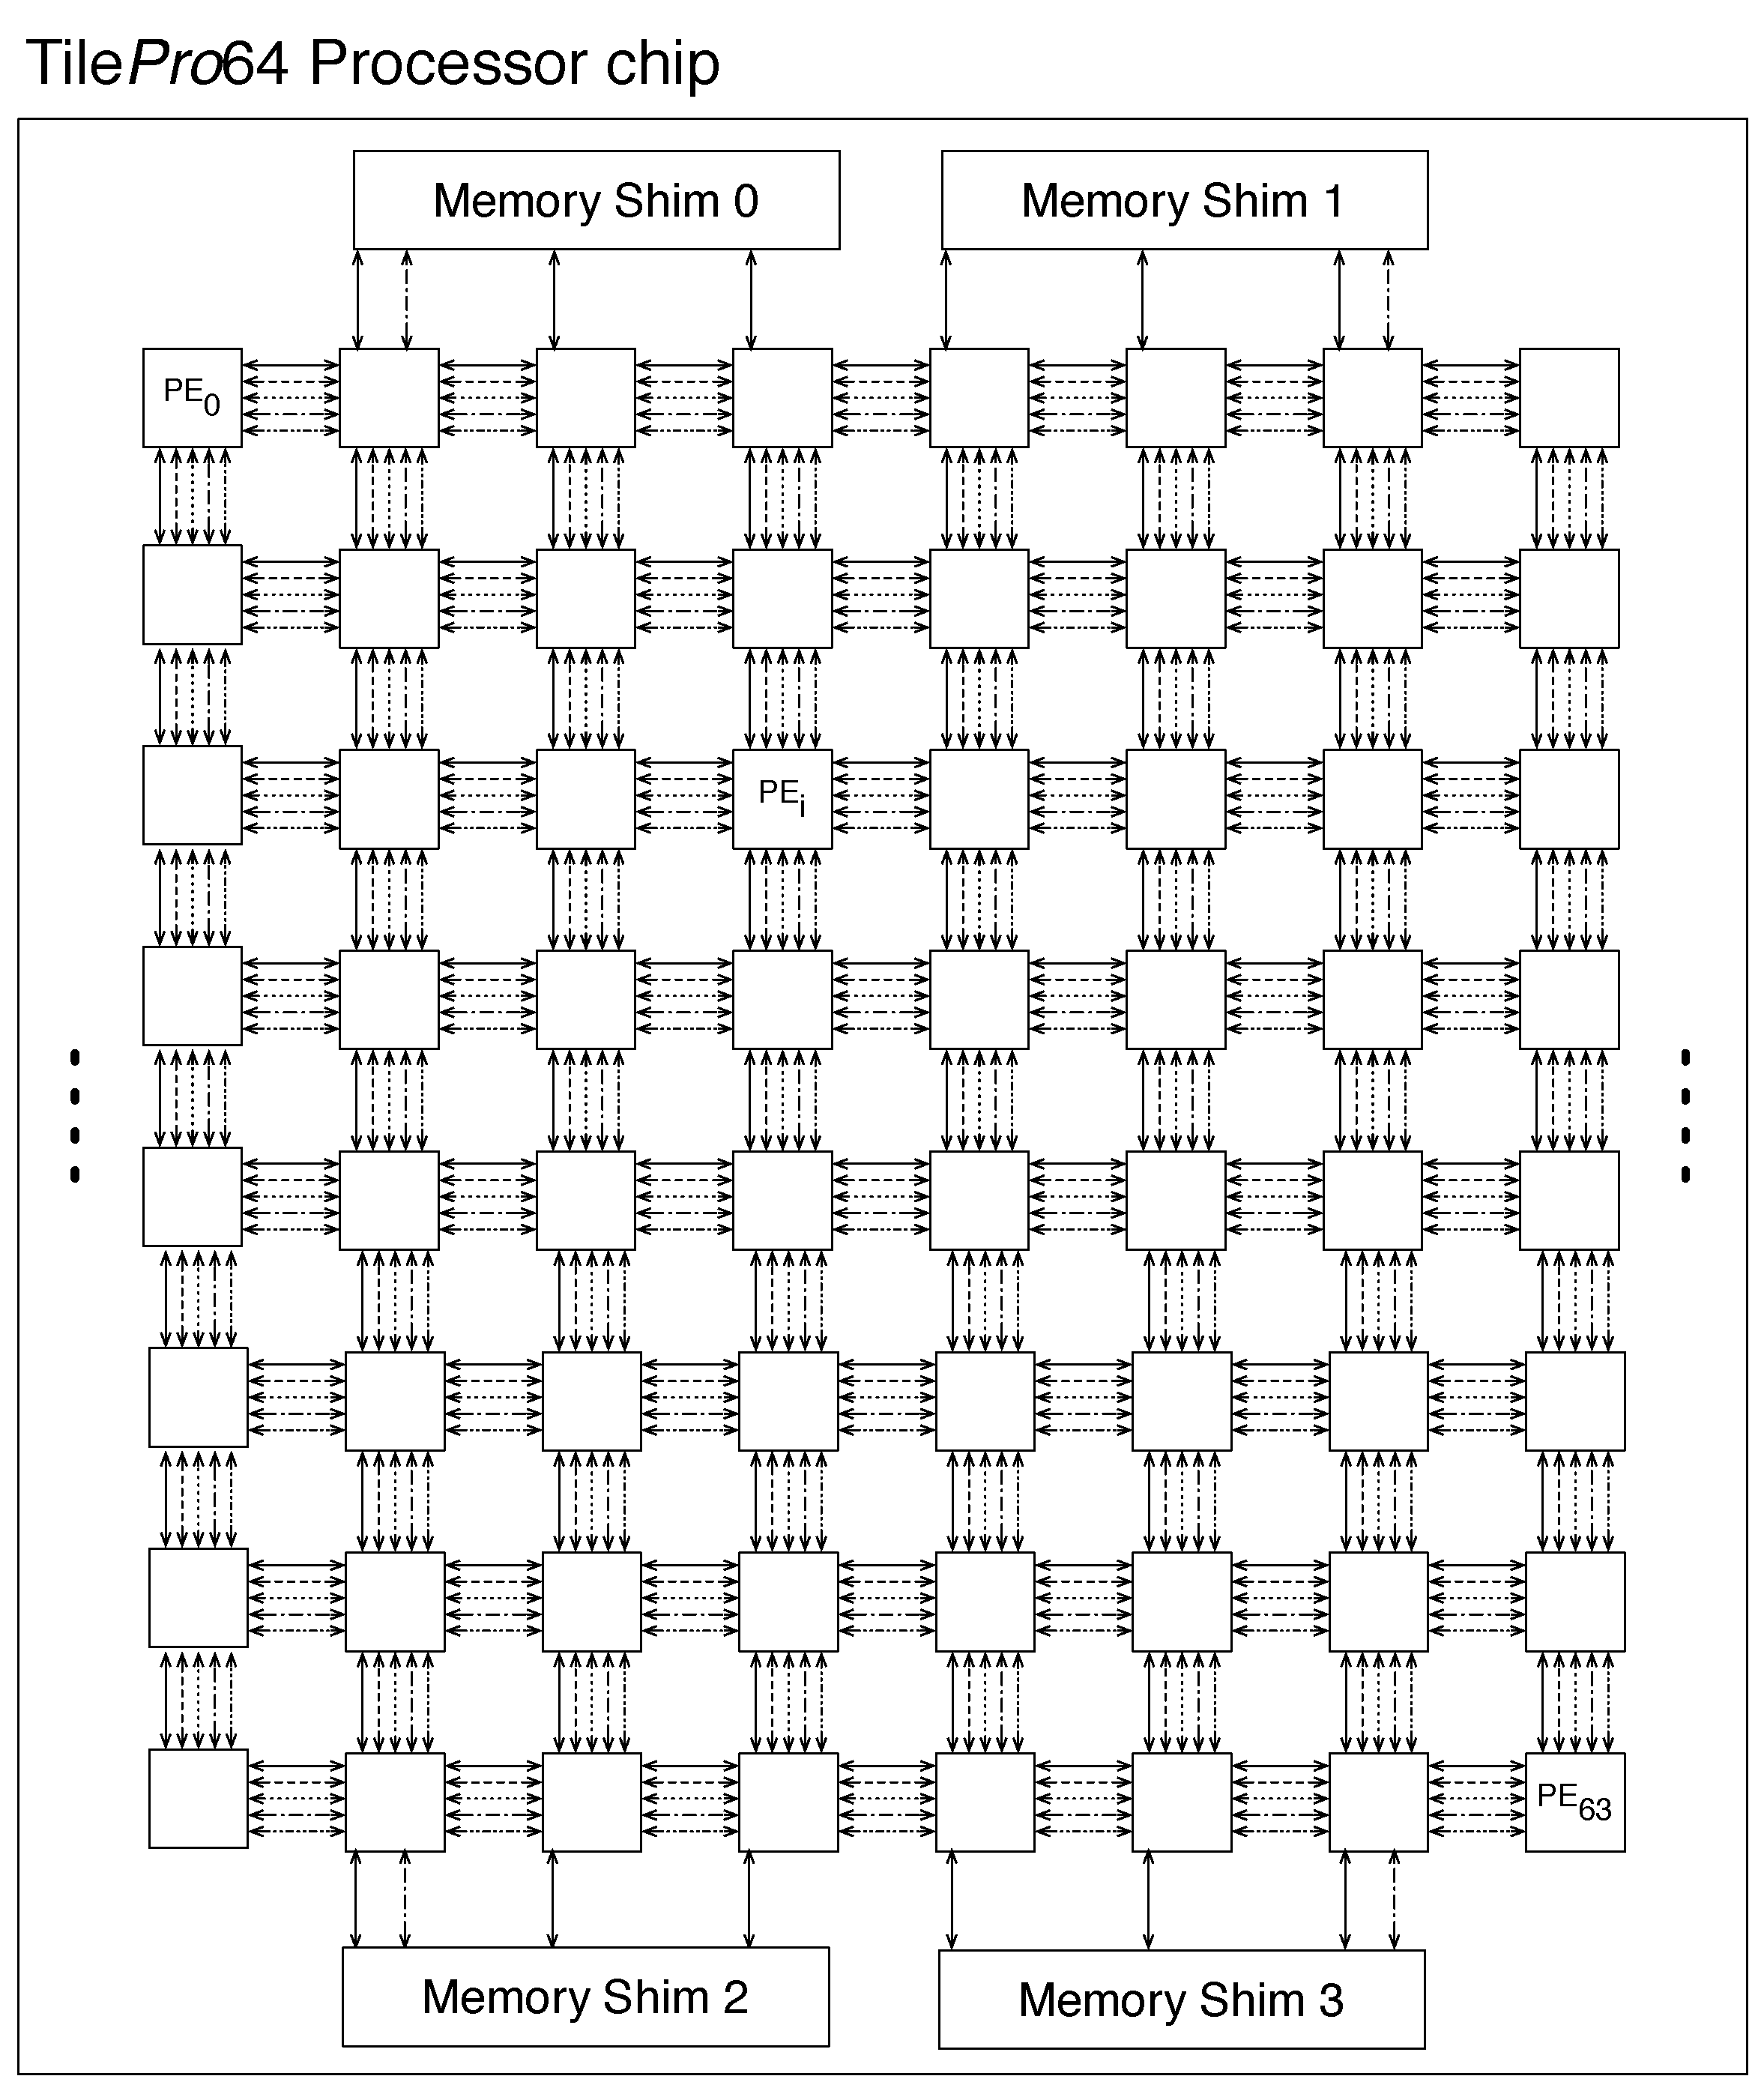
\includegraphics{schema_iMesh.pdf}}
    \label{fig:iMesh}
  \end{subfigure}
  \hspace{1ex}
  \begin{subfigure}[b]{.5\textwidth}
    \centering
    \resizebox{\columnwidth}{!}{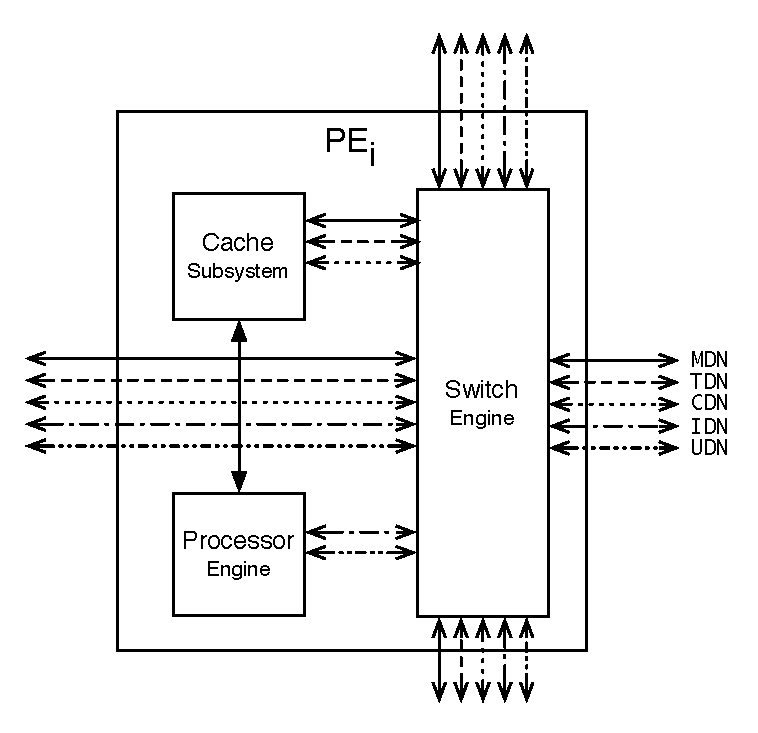
\includegraphics{schema_iMesh_tile.pdf}}
    \label{fig:iMesh_tile}
  \end{subfigure}     
  \caption[Schema del processore Tilera \tile]{Rappresentazione parziale del processore \tile\ con il dettaglio dell'architettura di un singolo Processing Element}
  \label{fig:tilera}
\end{figure}

\subsubsection{User Dynamic Network}
\label{sct:intro_arch_udn}
La UDN \`e collegata direttamente tra CPU e l'unit\`a di switching del PE. Sono disponibili quattro flussi UDN, nella CPU esistono altrettante code verso le quali sono direzionati i pacchetti del flusso corrispondente; esiste inoltre una quinta coda, detta Catch-All, per qualsiasi altro flusso diverso dai quattro precedenti. Le code di demultiplexing UDN sono collegate direttamente alla Unit\`a di Esecuzione delle Istruzioni della CPU. L'accesso ai flussi UDN avviene tramite letture o scritture a 4 registri generali riservati alla UDN. Il programmatore ha possibilit\`a di uso della UDN per mezzo della libreria C messa a disposizione da Tilera, tuttavia, le vere richieste di scrittura e lettura alla UDN sono effettuate per mezzo di istruzioni assembler, come mostrato nel codice~\ref{lst:udn_eg}.
%% udn0 - udn3 <----> 59 - 62
\begin{lstlisting}[float = b, basicstyle = {\small \ttfamily}, commentstyle={\rmfamily \itshape \footnotesize}, caption = {Istruzioni assembler per accedere alla UDN}, label = {lst:udn_eg}]
add r59, r5, r6 // Somma r5 a r6 e invia il risultato 
                // sul primo flusso UDN
add r5, r6, r60 // leggi una parola dal secondo flusso UDN,
                // sommala a r6 e scrivi il risultato in r5
\end{lstlisting}
L'attesa in seguito all'invocazione di un invio, o di una ricezione, \`e caratterizzata da un basso consumo di energia e da zero latenza alla sveglia. Si osserva che l'attesa in ricezione avviene quando non esistono dati nella coda del flusso UDN specificato. \`E possibile anche l'attesa in seguito all'invio quando la rete non \`e in grado di consumare immediatamente il pacchetto.

In conclusione la rete UDN offre molti vantaggi (bassissima latenza nella comunicazione PE-to-PE, zero latenza nella sveglia, bassi consumi) e presenta alcune limitazioni (il firmware realizza quattro flussi, la dimensione massima dei pacchetti \`e fissata a circa 118 parole). Tale servizio pu\`o perci\`o risultare interessante, e la documentazione ufficiale Tilera lo precisa \cite{ug205}, per ottimizzare l'implementazione di operazioni critiche per le prestazioni, mentre \`e raccomandato l'uso della memoria condivisa per la maggior parte delle comunicazioni. Nel caso di computazioni di grana fine, i meccanismi chiave sono quelli di sincronizzazione e comunicazione tra processi, la cui ottimizzazione fornisce miglioramenti notevoli alle prestazioni.

\subsection{Architettura della memoria principale}
\label{sct:intro_arch_memory}
Esistono quattro controllori della memoria principale collegati ai PE sul bordo superiore e inferiore della mesh. Le pagine di memoria condivisa hanno dimensione 64KB e sono allocate in modo interleave, in parti di 8KB, nei controllori di memoria (``stripped main memory mode''), tale configurazione rende uniforme l'accesso ai controllori di memoria bilanciando il carico di richieste. \`E possibile configurare l'allocazione delle pagine in specifici controllori. \tile\ definisce un modello \emph{rilassato} di consistenza della memoria, in altre parole l'ordinamento delle operazioni di store non \`e totale. Valgono le seguenti due propriet\`a:
\begin{itemize}
  \item la sequenza delle istruzioni originale del programma pu\`o essere modificata a tempo di compilazione, come risultato di ottimizzazioni. 
\item le operazioni di store eseguite da un PE appaiono visibili simultaneamente a tutti gli altri PE, ma possono diventare visibili al PE che ha emesso la scrittura prima che avvenga la visibilit\`a globale.
\end{itemize}       
L'architettura mette a disposizione un'istruzione di barriera di memoria, chiamata anche \emph{memory fence}, la quale stabilisce un ordinamento tra le istruzioni di memoria, altrimenti non ordinate: le operazioni di memoria nel programma prima dell'istruzione barriera di memoria, sono rese globalmente visibili prima di qualsiasi operazione dopo la barriera di memoria.

\subsection{Architettura del sottosistema di memoria cache}
\label{sct:intro_arch_cache}
La cache L1 \`e divisa nella parte istruzioni (L1i) e nella parte dati (L1d), la prima ha dimensione 16KB con blocchi di 64B, la seconda ha dimensione 8KB con blocchi di 16B. L'allocazione dei blocchi nelle due parti L1 avviene solo fault in lettura, le scritture sono write through. La cache L2 ha dimensione 64KB, blocchi di 64B e l'allocazione dei blocchi avviene con fault sia in lettura che in scrittura; la politica di scritture \`e write back.

La coerenza della memoria cache \`e garantita automaticamente, per mezzo del firmware della macchina. \`E possibile configurare la macchina in diverse modalit\`a:
\begin{itemize}
\item memoria coerente nelle cache;
\item memoria non coerente nelle cache, \`e onere del programmatore dell'applicazione garantire la coerenza mediante operazioni di flush e di deallocazione (\`e definita solo una primitiva che invalida il blocco nel PE che ha eseguito la primitiva stessa);
\item non uso della gerarchia cache.
\end{itemize}
La coerenza automatica si basa su invalidazione, l'implementazione \`e \emph{Directory-based}. In particolare la tabella Directory \`e implementata in modo distribuito nei PE della macchina.
Per un certo blocco di cache $b$ viene usato il termine Home con il consueto significato nei protocolli di coerenza cache: il PE che \`e Home per il blocco $b$ detiene e gestisce le informazioni di coerenza della cache di $b$, e invia messaggi di invalidazione quando necessario. Un PE gestisce la coerenza, e contiene le entrate della directory, dei soli blocchi di cui \`e Home. 
Nell'architettura Tilera un PE Home per un certo blocco $b$ ha anche la caratteristica di possedere sempre la copia aggiornata di $b$ nella propria L2 (in un protocollo di coerenza tale PE verrebbe chiamato Owner di $b$ oltre che Home). Questo consente di poter vedere un terzo livello di cache distribuito sulle L2: se un PE esegue una lettura da memoria che risulta miss sia nella L1d che nella L2 locali, tale richiesta viene inoltrata al PE che \`e Home del blocco corrispondente, piuttosto che essere inviata direttamente alla memoria. \`E onere della L2 di tale PE rispondere alla richiesta: se il blocco \`e allocato allora viene inviata immediatamente la risposta contenente il valore del blocco, altrimenti viene inoltrata la domanda di trasferimento alla memoria principale, e successivamente il messaggio di risposta al PE richiedente. Ne segue una caratterizzazione dei due livelli di cache: L1 \`e una cache privata per la propria CPU, la L2 \`e una cache condivisa con gli altri PE, in quanto pu\`o contenere sia blocchi acceduti dalla CPU locale, che blocchi di cui \`e Home e per i quali ha ricevuto una richiesta da un altro PE.
 
Lo schema con cui i blocchi di memoria vengono associati ai PE Home \`e dinamico e pu\`o essere controllato dal programmatore in modo da ottimizzare la specifica computazione, ad esempio rendendo massima la localit\`a delle informazioni nei PE. Sono disponibili tre modi per definire l'homing:
\begin{description}
\item [Local Homing] \`e la modalit\`a predefinita per lo stack dei processi e threads. Una pagina di memoria \`e Home nel PE che ha effettuato l'accesso. Ne segue che in tale modalit\`a tutti gli accessi sono diretti ai controllori di memoria e non viene usato il meccanismo di L3 cache distribuito nelle cache L2 degli altri PE. Ci\`o \`e utile per dati privati in quanto non trarrebbero vantaggio dall'uso della cache di una altro PE come L3.
\item [Hash-for-Home] \`e la modalit\`a predefinita per tutti gli altri dati del processo. Una pagina di memoria viene homed in modo sparso nei PE della macchina con granularit\`a di un blocco L2. Tale dispersione delle pagine di memoria nella cache dei PE consente una distribuzione uniforme del traffico nelle reti del chip e un effettivo bilanciamento del traffico di richieste alla memoria tra l'insieme dei PE.
\item [Remote Homing] per una generica pagina di memoria viene impostato il corrispondente PE Home. Tale PE \`e anche chiamato L3 per la pagina. Le richieste di accesso ad un qualsiasi blocco interno alla pagina, da parte di altri PE, vengono inoltrate al PE Home; quest'ultimo ha l'onere di rispondere con il trasferimento del blocco, eventualmente effettuando l'accesso alla memoria principale se il blocco non \`e presente nella sua L2. Tale configurazione \`e utile con strutture dati condivise, il cui accesso avviene con uno schema produttori-consumatore. Configurare la pagina dell'oggetto in questione come Home nel PE che esegue il consumatore aumenta la localit\`a degli accessi di tale processo, il quale si trova direttamente nella propria L2 la struttura modificata dai produttori. Le scritture effettuate dai produttori, infatti, sono write through nella cache del PE Home.
\end{description}
